\section{Predecessors: Walrasian and non-Walrasian equilibria}


\subsection{Non-walrasian equilibrium models}

Spillover effects

\begin{equation*}
\begin{aligned}
& \underset{C, L}{\max}
& & U = C ^ { \alpha } ( 1 - L ) ^ { 1 - \alpha } \\
& \text{s.t}
& & P \cdot C \leq W \cdot L + \pi
\end{aligned}
\end{equation*}


\begin{equation*}
    \mathcal{L} = C ^ { \alpha } ( 1 - L ) ^ { 1 - \alpha } + \lambda(P \cdot C \leq W \cdot L + \pi)
\end{equation*}



$$
\text{MRS}_{Z, c} = \frac{w}{p}
$$

$$
\frac{1 - \alpha}{\alpha} \cdot \frac{C}{1 - L}
$$


The notional consumption function (unrestricted):
\begin{equation}
    \Tilde{C} = \alpha \frac { W \cdot 1 + \pi } { P }
\end{equation}


Notional labour supply:
\begin{equation}
    \Tilde{L} = 1 - ( 1 - \alpha ) \frac { W \cdot 1 + \pi } { W }
\end{equation}


An additional constraint where:
$$
L \leq \Bar{L}_0
$$

\begin{equation}
    L ^ { * } = \min \left\{ \overline { L } _ { 0 } , \Tilde{L} \right\}
\end{equation}

\begin{equation}
    C ^ { * } = \min \left\{ \overline { Y } _ { 0 } , \Tilde{C} \right\} = \left\{ \alpha \frac { W \cdot \overline { L } _ { 0 }  + \pi } { P }, ... \right\}
\end{equation}

\subsubsection*{Microeconomic Foundations}
\paragraph{Assumptions}
\begin{enumerate}
    \item No rationed agents on both sides of the market
    \item Rationing scheme is non-manipulable
    \item Markets are perfectly competitive
\end{enumerate}

\subsubsection*{Partial equilibrium}
Partial equilibrium exists in the minimum of notional supply and demand, look at the slides

\subsubsection*{General Equilibrium}

$$
P = \left[ P_1, P_2, \dots, P_n  \right]
$$

$$
\mathbf{X} = \Downarrow (P)
$$

$$
\mathbf{X^*} = \Downarrow X (\mathbf{P, \overline{Z}})
$$

\subsection*{An Illustrative Model}

\subsubsection*{Assumptions}
\begin{enumerate}
    \item $n = 1$ --- Number of goods in the economy
    \item $\alpha = 1$ --- Labour does not give any disutility
    \item $\Phi = 0$ --- No fixed costs
    \item $\Psi = 0$ --- No costs to change prices  - Menu Costs
    \item $M = \infty$ --- Number of firms producing each good
    \item $A = 1$
    \item Population = 1
\end{enumerate}

\subsubsection*{The Household Problem}

\begin{equation*}
\begin{aligned}
& \underset{C, M}{\max}
& & U = C ^{\gamma} \cdot \frac{M}{P}^{1 - \gamma} \\
& \text{s.t}
& & M_E + wL + \pi -T = M + PC \\
& & &  L  = \min \left\{ \overline { N }  , 1 \right\}
\end{aligned}
\end{equation*}

Since Labour does not gives any disutility, households wants to work as much as possible. If $\Bar{N} < 1$ the household is rationed in the labour market and can only work less than what they want. 


The demand for consumption goods:

\begin{equation}
    C = \gamma \frac{M_E + wL + \pi -T}{P}
\end{equation}

The notional demand for consumption is given by the following equation, when $L = 1$:

\begin{equation}
   \Tilde{C} = \gamma \frac{M_E + w \cdot 1 + \pi -T}{P}
\end{equation}


The effective demand is given by the following expression, which is the minimum between the notional demand for consumption goods and the case where $L = \Bar{N}$:
\begin{multline}
    \Tilde{C} = \min \left\{ \Tilde{C}, \gamma \frac{M_E + w \overline{N} 1 + \pi -T}{P} \right\} = \\
      \gamma \left( \frac{M_E - T}{P} + Y^* \right) \implies \\
     \gamma \frac{M_E}{P} + \gamma \left( Y^* - \frac{T}{P} \right)
\end{multline}

Where $\gamma$ represents the marginal propensity to consume.


\subsubsection*{Government}
As opposed to households, the government can never be rationed

$$
\Tilde{G} = G^* = \overline{G}
$$


The total demand is given by Household consumption $C^*$ plus Government Consumption $G^*$
$$
D^* = C^* + G^* = \gamma \left( \frac{M_E - T}{P} + Y^* \right) + \overline{G}
$$

\[ Y^* = \left\{ \begin{array}{ll}
         f(1) & \mbox{if $L^* = 1$};\\
        f(\overline{N}) & \mbox{if $L^* = \overline{N}$}.\end{array} \right. \] 
        
        
        
$$
L^* = \min \left\{ \overline{N}, 1 \right\}
$$

\subsubsection*{Firms}

\begin{equation*}
\begin{aligned}
& \underset{\Pi}{\max}
& & \Pi = PY - WN \\
& \text{s.t}
& & Y = 1N^\beta \\
& & &  Y \leq D \\
& &  & N \leq 1
\end{aligned}
\end{equation*}

$$
TC = WN = W \cdot Y^{\frac{1}{\beta}}
$$

$$
MC  = \frac{1}{\beta} W \cdot Y^{\frac{1 - \beta}{\beta}}
$$

$$
P = MC
$$

The notional supply of goods
$$
\Tilde{Y} = \left( \frac { P \cdot \beta} { W } \right) ^ { \frac { \beta } { 1 - \beta } }
$$

Notional demand for labour
$$
\Tilde{N} = \left( \frac { W } { \beta \cdot P } \right) ^ { \frac { 1 } { 1 - \beta } }
$$

\subsubsection*{If the firm is rationed in the goods market: }

$$
\Tilde{Y} > \overline{D} = Y^*
$$

Which means that we have excess supply ?


$$
1 N^{\beta} = \overline{D} \implies N = \left( \frac{D}{1} \right)^{\frac{1}{\beta}} 
$$


Effective Labour Demand
$$
N^* = \min \left\{ \left( \frac { W } { \beta \cdot P } \right) ^ { \frac { 1 } { 1 - \beta } },  \left( \frac{D}{1} \right)^{\frac{1}{\beta}}   \right\}
$$

\subsubsection*{If the firm is rationed in the labour market: }

$$
\Tilde{N} > \Tilde{L} = 1 = L^*
$$


$$
Y = 1(N^*)^\beta = 1
$$

Effective labour Supply
$$
Y^* = \min \left\{ \left( \frac { P \cdot \beta} { W } \right) ^ { \frac { \beta } { 1 - \beta } }, 1   \right\}
$$

Check slides for more regimes

\subsection*{Keynesian Unemployment Regime}
The Keynesian regime exhibits excess supply in both markets.
$$
P > P_w
$$

$$
\frac{W}{P} > \left( \frac{W}{P} \right)_W
$$

$$
D^* = \gamma \left( \frac{M_E - T}{P} + Y^* \right) + \overline{G}
$$

$$
N^* = D^{* \frac{1}{\beta}} < \Tilde{L} = 1
$$

\begin{align}
    Y^* = D^* \implies \\
    &  Y^* = \gamma \left( \frac{M_E - T}{P}  \right) + -  \gamma Y^* \overline{G} \implies \\
\end{align}

Autonomous demand is given by:
$$
\Omega \equiv \gamma \frac{M_E - T}{P} + \overline{G}
$$

So we have: 

$$
Y^* = \frac{\Omega}{1 - \gamma}
$$

$$
N* = \left( \frac{\Omega}{1 - \gamma}  \right)^{\frac{1}{\beta}} < 1
$$

$$
\frac{\partial Y^*}{\partial G^*} = \frac{1}{1 - \gamma} > 1
$$

$$
\frac{\partial Y^*}{\partial M_E} = \frac{\gamma}{(1 - \gamma) P} > 0
$$

\clearpage

\subsection*{Classical Unemployment Regime}
With classical unemployment we have excess supply of labor and an excess demand for goods. 

$$
N^* = \Tilde{N} = \left( \frac { W } { \beta \cdot P } \right) ^  { - \frac { 1 } { 1 - \beta }} < \Tilde{L} = 1
$$
\begin{equation}\label{YStar}
    Y^* = 1 \cdot N^{*\beta} = \left(  \frac{w}{\beta P} \right)^{ - \frac{1}{1 - \beta}} 
\end{equation}

We can rewrite the previous equation as a function of real wage instead of nominal wage by defining $\omega$;
$$
\omega \equiv \frac{w}{P}
$$

Thus from \ref{YStar} we have: 
$$
\left( \frac{\omega}{\beta} \right) ^{ - \frac{\beta}{1 - \beta}}
$$




\paragraph{Policies}

\begin{align*}
    \frac { \partial Y ^ { * } } { \partial \overline { G } } = 0 && \frac { \partial Y ^ { * } } { \partial M_E } = 0 
    &  & \frac{\partial Y^*}{\partial \omega} = - \frac{Y^*}{1 - \beta} * \frac{\beta}{\omega} < 0
\end{align*}

By looking at the partial derivatives we see that government consumption through $\overline{G}$ is ineffective and will not change the level of unemployment, the same goes for monetary policy through $M_E$. Firms are already selling as much as they want at the given prices. The problem is that the prices is not???

There is excess demand in the economy and therefore Keynesian demand stimulating policies would not work. 

However, the only thing that would work is price and income policies to affect the real wage. This is clear by looking at the $\tfrac{\partial Y^*}{\partial \omega}$ which is negative. This means that if you could reduce the real wage production could be stimulated because they are too high. Examples of such policies could be labour market regulations and so on.  Such policies would not work in a Keynesian regime as the real wage do not affect output. 



\subsubsection*{Suppressed Inflation}
In the suppressed inflation unemployment regime we have excess demand in both markets; 

$$
\Tilde{L} < \Tilde{N} \land \Tilde{Y} < \Tilde{D}
$$
$$
\Tilde{N} > \Tilde{L} = 1 \implies L^* = 1
$$

$$
Y^* = 1 \cdot N^{* \beta} = 1
$$

$$
Y^* = C^* + \overline{G} \implies C^* = 1 - \overline{G}
$$

\clearpage


\paragraph{Putting everything together --- Delimitation of the regimes}
\begin{table}[ht]
\begin{tabu} to \linewidth{|X[-2.5,c,m]|X[c,m]|X[c,m]|}
\tabucline-
    \backslashbox{Labour Market}{Product Market} & $$\Tilde{Y} > \Tilde{D}$$ & $$\Tilde{Y} < \Tilde{D}$$  \\ \hline
    $$\Tilde{L} > \Tilde{N}$$  & Keynesian Unemployment & Classical Unemployment \\ \hline
    $$\Tilde{L} < \Tilde{N}$$ & Not possible due to the absence of stockage & Suppressed Inflation   \\ \hline
\end{tabu}
\caption{Unemployment regimes}
\end{table}

\begin{figure}[h!]
    \centering
    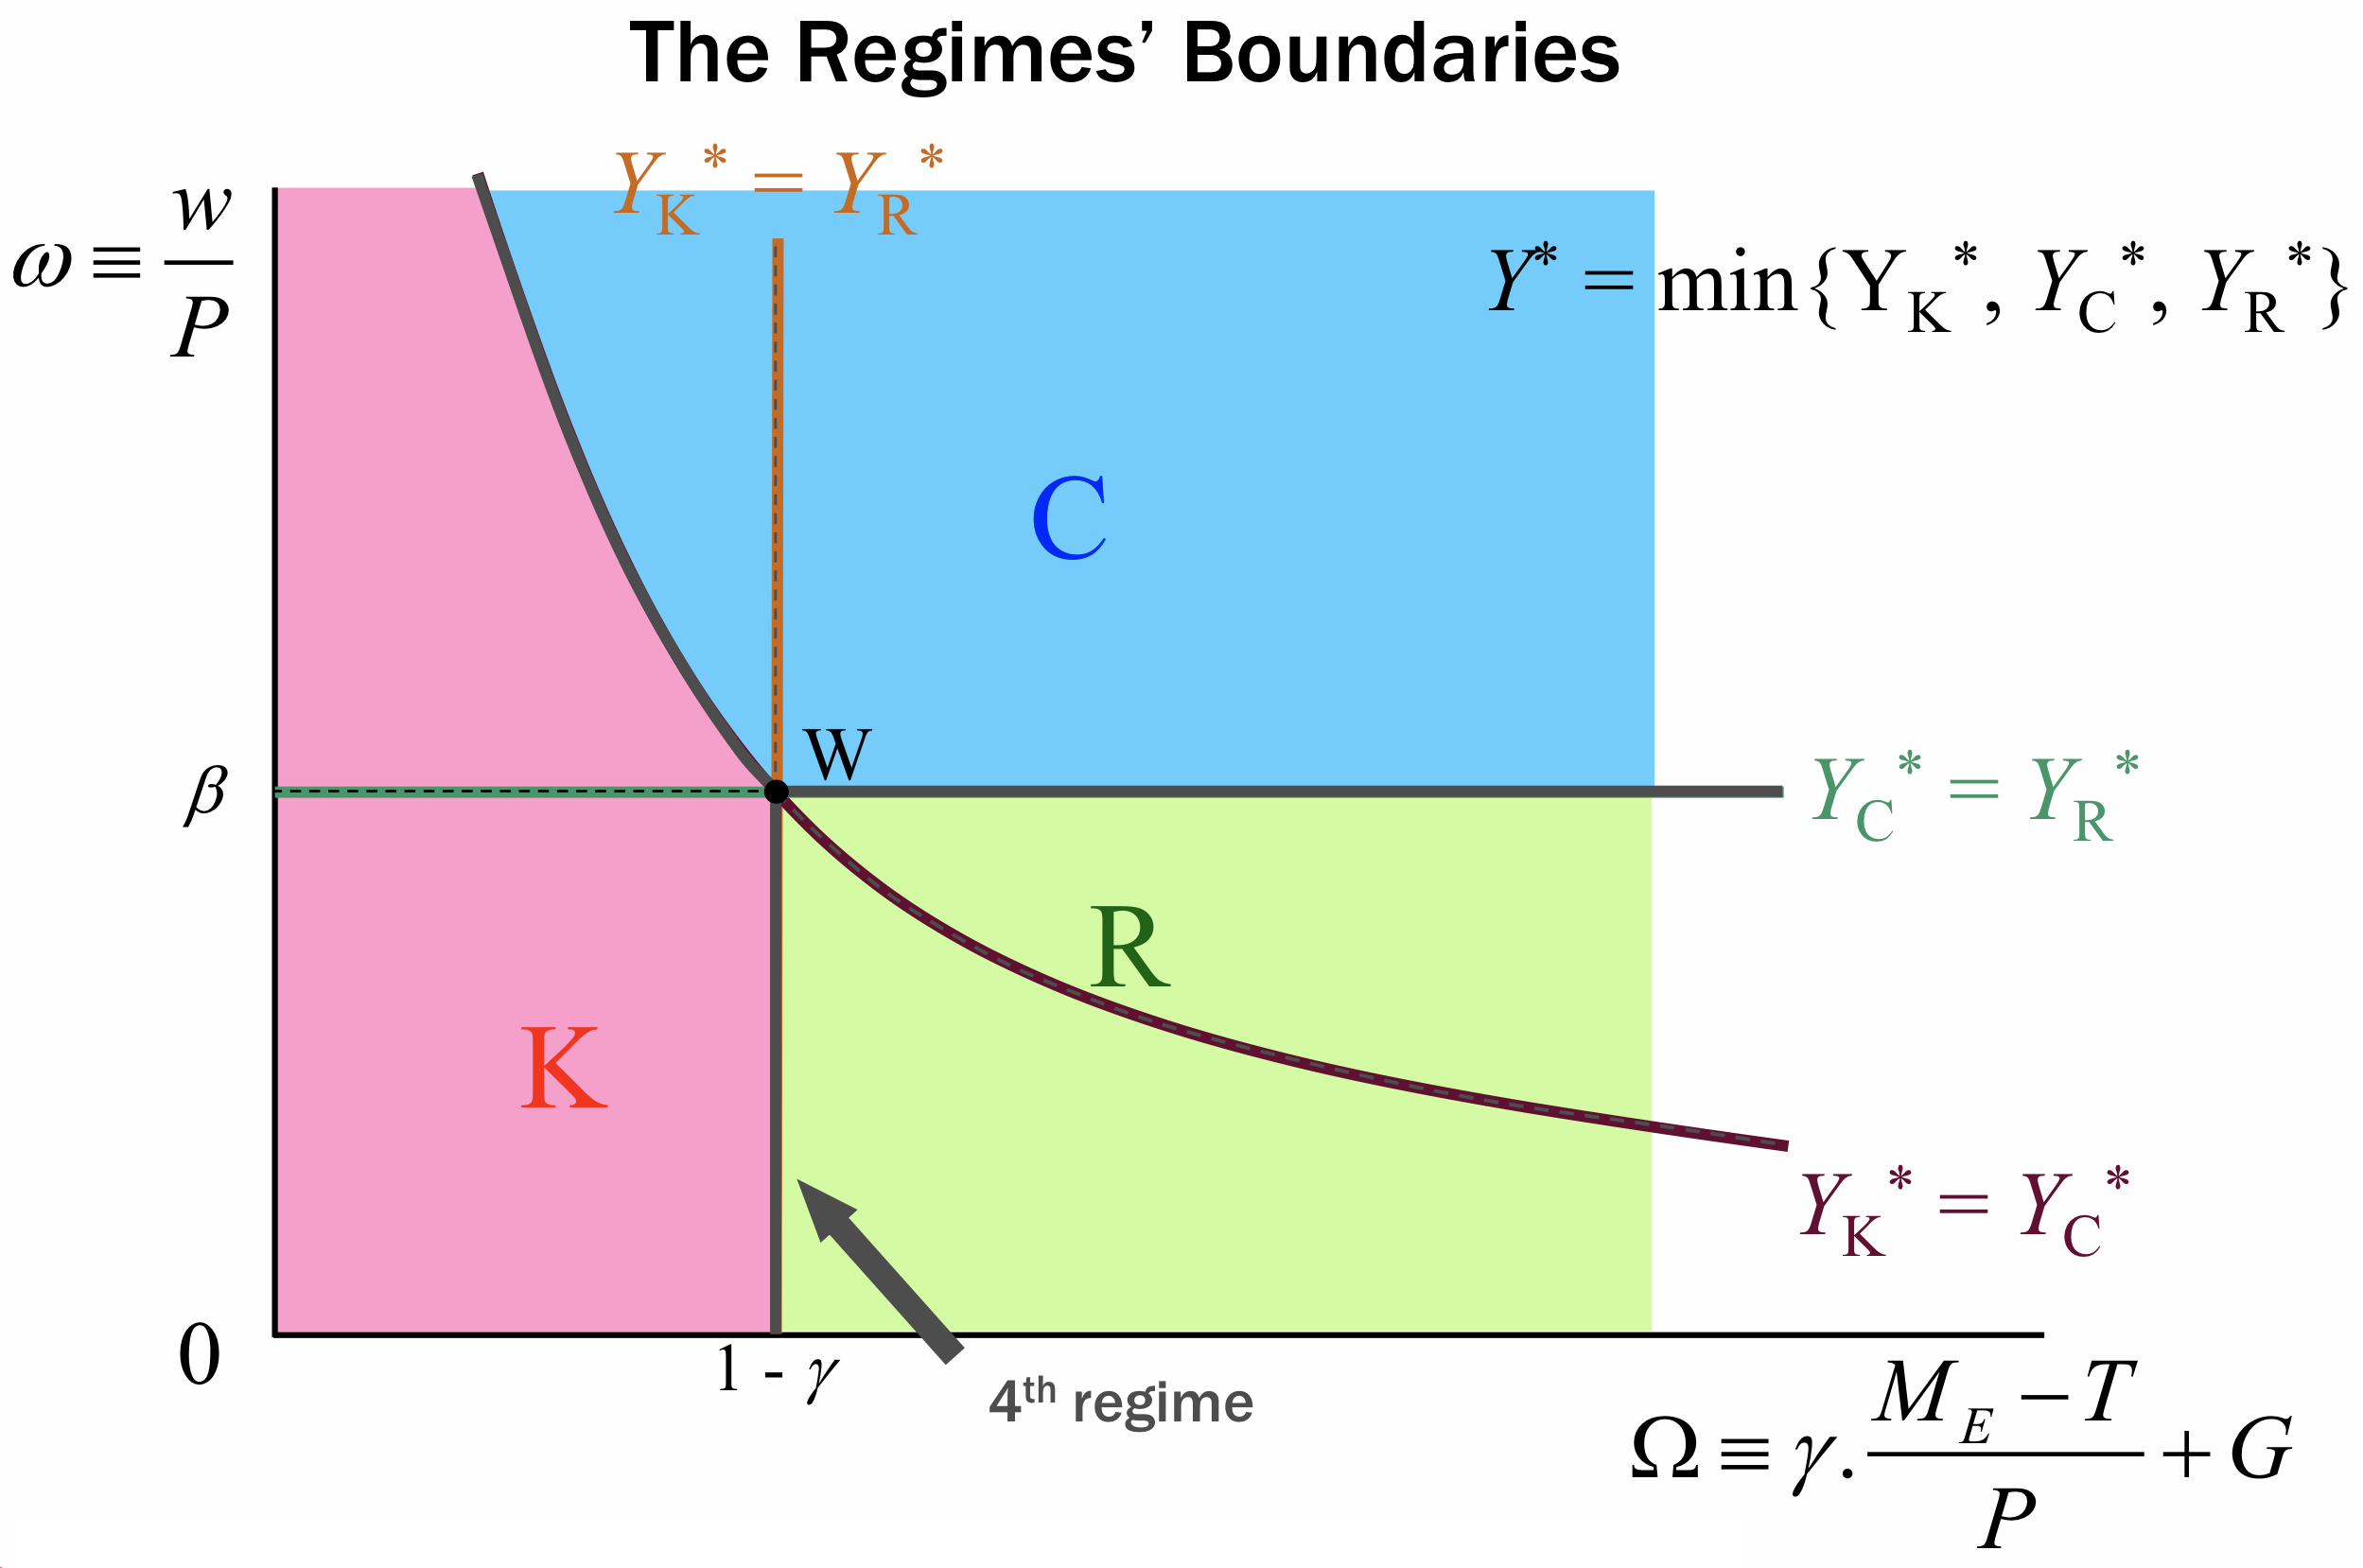
\includegraphics[width=\textwidth]{4_0_New_Keynesian_School/regime_boundaries.png}
    \caption{Regime Boundaries}
    \label{fig:my_label}
\end{figure}
\clearpage
